%
% For tracking purposes - this is V2.0 - May 2012

\documentclass{sig-alternate-05-2015}

\usepackage[colorinlistoftodos,obeyFinal]{todonotes}                           
%\usepackage{caption}
\usepackage{fainekos-macros}
\usepackage[]{algorithm2e}
\usepackage{amsmath} % assumes amsmath package installed
\usepackage{amssymb}  % assumes amsmath package installed
\usepackage{graphicx}
\usepackage{tikz}
\usetikzlibrary{arrows}
\usepackage{ifthen}
\usepackage{mathtools}
\usepackage{stmaryrd}
\usepackage{csquotes}
\usepackage{xargs}                      % Use more than one optional 
\usepackage{subcaption}
%\usepackage[pdftex,dvipsnames]{xcolor}  % Coloured text etc. 
\usepackage[obeyFinal]{todonotes}

\newcommand{\rob}{\rho}
\newcommand{\robf}{\rho_{\formula}}
\newcommand{\robfa}{\rho_{\formula_1}}
\newcommand{\robfb}{\rho_{\formula_2}}
\newcommand{\srob}{\tilde{\rob}}
\newcommand{\srobf}{\srob_\formula}
\newcommand{\smax}{\widetilde{\max}}
\newcommand{\smin}{\widetilde{\min}}
\newcommand{\sdist}{\mathbf{dist}_\varepsilon}

\newcommand{\sd}{\rho}
\newcommand{\bs}[2]{\ll\!#1,#2\!\gg}
\newcommand{\rd}[2]{\ll\!#1,#2\!\gg_\Re}
\newcommand{\rs}[2]{\ensuremath{\llbracket #1,#2 \rrbracket}}
\newcommand{\cl}[1]{\overline{#1}}
\newcommand{\Ltf}{\Lc_t(\formula)}
\newcommand{\Ltnp}{\Lc_t(\lnot p)}
\newcommand{\Ltp}{\Lc_t(p)}
\newcommand{\Lrf}{\Lc_{\Re_\Fc}}

% Control spacing...
%\setlength{\marginparwidth}{4cm}
%\setlength{\textfloatsep}{2pt}
%\linespread{0.97}
%\thickmuskip=0mu

\begin{document}

\CopyrightYear{2017} \setcopyright{acmcopyright}
\conferenceinfo{ICCPS '17,}{April 18--21, 2017, Pittsburgh, Pennsylvania, USA.}
\isbn{978-1-4503-3955-1/16/04}\acmPrice{\$15.00}
\doi{http://dx.doi.org/10.1145/2883817.2883841}
%Authors, replace the red X's with your assigned DOI string.

\title{Smooth Operator: Control Using the Smooth Robustness of Temporal Logic}

\author{
	% 1st. author
	\alignauthor
	Three little piggies\\
	\affaddr{Department of Electrical and Systems Engineering}\\
	\affaddr{University of Pennsylvania, Philadelphia, PA, USA}\\
	\email{\{piggies1,2,3\}@seas.upenn.edu}%
}


\maketitle
\begin{abstract}
 
 
 
 
 Cyber-Physical Systems must withstand a wide range of errors, from bugs in their software to attacks on their physical sensors.
 Given a formal specification of their desired behavior in Metric Temporal Logic (MTL), the robust semantics of the specification provides a notion of \textit{system robustness} that can be calculated directly on the output behavior of the system, without explicit reference to the various sources or models of the errors.
 The robustness of the MTL specification has been used both to verify the system offline (via robustness minimization) and to control the system online (to maximize its robustness over some horizon).
 Unfortunately, the robustness objective function is difficult to work with: it is recursively defined, non-convex and non-differentiable.
 In this paper, we propose smooth approximations of the robustness. 
 Such approximations are differentiable, thus enabling us to use powerful off-the-shelf gradient descent algorithms for optimizing it.
 By using them we can also offer guarantees on the performance of the optimization in terms of convergence to minima.
 We show that the approximation error is bounded to any desired level, and that the approximation can be tuned to the specification.
 We demonstrate the use of the smooth robustness to control two quad-rotors in an autonomous air traffic control scenario, and for temperature control of a building for comfort.
\end{abstract}

\section{Introduction}
\label{sec:intro}

New:
nonlinear control with mpc on feedback linearized dynamics with state estimation error, input constraints, state constraints
	feedback linearization but no state constraints and identity T, no state uncertainty
	
state constraints
recursive feasibility with time-varying error sets

\textbf{Notation}.
Given two subsets $A,B$ of $\Re^n$, define their \textit{Minkowski sum} to be $A\oplus B \defeq \{a+b \such a\in A, b\in B\}$.
Define their Pontryagin difference to be $A\ominus B = \{c \in \Re^n \such c+b \in A \forall b \in B\}$
\section{Robustness of MTL formulae}
\label{sec:robust semantics}

Consider a discrete-time dynamical system $\Sys$ given by 
\begin{equation}
\label{eq:xt}
x_{t+1} = f(x_t,u_t)
\end{equation}
where $x \in X \subset \Re^n$ is the state of the system and $u \in U \subset \Re^m$ is its control input.
The system's initial state $x_0$ takes value from some initial set $X_0 \subset \Re^n$.
Given an initial state $x_0$ and a finite control input sequence $\inpSig = (u_0,\ldots, u_{T-1}), u_t \in U$, a \textit{trajectory} of the system is the unique sequence of states $\sstraj = (x_0,\ldots,x_T)$ s.t. for all $t$, $x_t$ is in $X$ and obeys \eqref{eq:xt}.
%We will use $\TDom$ to abbreviate the time domain $\{0,1,2,\ldots\}$.
All temporal intervals that appear in this paper are implicitly discrete-time, e.g. $[a,b]$ means $[a,b] \cap \Ne$. 
The set $\{0,1,\ldots,T\}\subset \Ne$ will be abbreviated as $\TDom$.
For an interval $I \subset \Ne$, let $t+I = \{t+a \such a \in I\}$.
The set of subsets of a set $S$ is denoted $\Pc(S)$.
The signal space $\SigSpace$ is the set of all signals $\sstraj: \TDom \rightarrow X$.
The max operator is written $\sqcup$ and min is written $\sqcap$.

\subsection{Metric Temporal Logic (MTL)}
\label{sec:mtl}
The controller of $\Sys$ is designed to make the closed loop system \eqref{eq:xt} satisfy a specification expressed in MTL~\cite{Ouaknine08_RecentResultsMTL}.
Formally, let $AP$ be a set of atomic propositions, which can be thought of as point-wise constraints on the state of the system.
An MTL formula $\formula$ is built recursively from the atomic propositions using the following grammar:
\[\formula \defeq \top|p|\neg \formula | \formula_1 \land \formula_2 | \formula_1 \until_I \formula_2\]
where $I \subset \Re$ is a time interval.
Here, $\top$ is the Boolean True, $p$ is an atomic proposition, $\neg$ and $\land$ are the Boolean negation and AND operators, respectively, and $\until$ is the Until temporal operator.
Informally, $\formula_1 \until_I \formula_2$ means that $\formula_1$ must hold \textit{until} $\formula_2$ holds, and that the hand-over from $\formula_1$  to $\formula_2$ must happen sometime during the interval $I$.
The disjunction ($\lor$), implication ($\implies$), Always ($\always$) and Eventually ($\eventually$) operators can be defined using the above operators.

Formally, the \textit{pointwise semantics} of an MTL formula define what it means for a system trajectory $\sstraj$ to satisfy the formula $\formula$.
Let $\Oc: AP \rightarrow \Pc(X)$ be an \textit{observation} map for the atomic propositions.
The boolean truth value of a formula $\formula$ w.r.t. the trajectory $\sstraj$ at time $t$ is defined recursively.
\begin{definition}[MTL semantics]
	\label{def:boolean sat}
	\begin{eqnarray*}
		\label{eq:boolean sat}
		(\sstraj,t) \models \top &\Leftrightarrow& \top
		\\
		\forall p \in AP, (\sstraj, t) \; \models_\Oc p &\Leftrightarrow& x_t \in \Oc(p)
		\\
		(\sstraj,t) \models_\Oc \neg \formula&\Leftrightarrow& \neg (\sstraj,t) \models_\Oc \formula
		\\
		(\sstraj,t) \models_\Oc  \formula_1 \land \formula_2&\Leftrightarrow& (\sstraj,t) \models_\Oc \formula_1 \land (\sstraj,t) \models_\Oc \formula_2
		\\
		(\sstraj,t) \models_\Oc \formula_1 \until_I \formula_2 &\Leftrightarrow& \exists t' \in t+I .  (\sstraj,t') \models_\Oc \formula_2  
		\\
		&& \, \land \forall t'' \in (t,t'), \;\; (\sstraj,t'') \models_\Oc \formula_1 
	\end{eqnarray*}
\end{definition}
As $\Oc$ is fixed in this paper, it is dropped from the notation.
We say $\sstraj$ satisfies $\formula$ if $(\sstraj,0) \models \formula$.
\textit{All formulas that appear in this paper have bounded temporal intervals: $ 0\leq \inf I < \sup I < +\infty$.}
To evaluate whether such a formula $\formula$ holds on a given trajectory, only a finite-length prefix of that trajectory is needed.
Its length can be upper-bounded by the \textit{horizon} of $\formula$, $hrz(\formula) \in \Ne$, calculable as shown in~\cite{Dokhanchi14_OnlineMonitoring}. 
For example, the horizon of $\always_{[0,2]}(\eventually_{[2,4]}p)$ is 2+4=6.

\subsection{Robust semantics of MTL}
\label{sec:rob sem}
Designing a controller that satisfies the MTL formula $\formula$\footnote{Strictly, a controller s.t. the closed-loop behavior satisfies the formula.} is not always enough.
In a dynamic environment, where the system must react to new unforeseen events, it is useful to have a margin of maneuverability.
That is, it is useful to control the system such that we \textit{maximize} our degree of satisfaction of the formula.
When unforeseen events occur, the system can react to them without violating the formula.
This degree of satisfaction can be formally defined and computed using the robust semantics of MTL.
Given a point $x \in X$ and a set $A \subset X$, $\dist(x,A) \defeq \inf_{a \in \cl{A}}|x-a|_2$ is the minimum Euclidian distance from $x$  to the closure $\cl{A}$ of $A$.
\begin{definition}[Robustness\cite{FainekosP09tcs}]
	\label{def:robustness estimate}
	The \emph{robustness} of $\varphi$ relative to $\sstraj$ at time $t$ is recursively defined as 
	\begin{eqnarray*}
		\label{eq:robustness estimate}
		\rob_{\top} (\sstraj,t) &=& +\infty
		\\
		\forall p \in AP, \;  \rob_{p} (\sstraj,t) &=& \left \lbrace \begin{matrix}
			\dist(\stPt_t, \stSet \setminus \Oc(p)), &\text{if } \stPt_t \in \Oc(p)
			\\
			-\dist(x_t, \Oc(p)), &\text{if } \stPt_t \notin \Oc(p)						
		\end{matrix} \right.
		\\
		\rob_{\lnot \formula} (\sstraj,t) &=& - \rob_{\formula} (\sstraj,t)
		\\
		\rob_{ \formula_1 \land \formula_2} (\sstraj,t) &=& \rob_{\formula_1} (\sstraj,t) \sqcap \rob_{\formula_2} (\sstraj,t) 
		\\
		\rob_{ \formula_1 \until_I \formula_2} (\sstraj,t) &=& \sqcup_{t' \in t+_{\TDom}I} \left(\rob_{\formula_2} (\sstraj,t') \bigsqcap \right.
		\\
		&& \left. \sqcap_{t'' \in [t,t')}   \rob_{\formula_1} (\sstraj,t'') \right) 
	\end{eqnarray*}
	When $t=0$, we write $\robf(\sstraj)$ instead of $\robf(\sstraj,0)$.
\end{definition}
The robustness is a real-valued function of $\sstraj$ with the following important property.
\begin{theorem} \cite{FainekosP09tcs}
	\label{thm:rob objective}
	For any $\sstraj \in \SigSpace$ and MTL formula $\formula$, 
	if $\robf(\sstraj,t) <0$ then $\sstraj$ violates the spec $\formula$ at time $t$, and if $\robf(\sstraj,t) > 0$ then $\sstraj$ satisfies $\formula$ at $t$. 
	The case $\robf(\sstraj,t) =0$ is inconclusive.
\end{theorem} 

Thus, we can compute control inputs by maximizing the robustness over the set of finite input sequences of a certain length.
The obtained sequence $\inpSig^*$ is valid if $\robf(\sstraj,t)$ is positive, where $\sstraj$ and $\inpSig^*$ obey \eqref{eq:xt}.
The larger $\robf(\sstraj,t)$, the more robust is the behavior of the system: intuitively, $\sstraj$ can be disturbed and $\robf$ might decrease but not go negative.

\section{Smooth approximation}
\label{sec:smooth apx}
\newcommand{\fe}{f_\varepsilon}

Let $\formula$ be an MTL formula with horizon $N$.
The goal of the present work is to solve the following problem $P_\rob$.
\begin{subequations}
	\label{eq:general_ctrl}
	\begin{align}
	P_\rob:\, \max_{\mathbf{u}}\, & \rob_{\formula}(\sstraj) - \gamma \sum_{k=0}^{N-1} l(x_{k+1},u_{k}) \label{eq:general ctrl obj}\\
	\text{s.t. } & x_{k+1} = f(x_k,u_k), \, \forall k=0,\dotsc,N-1 \label{eq:general ctrl dyn}\\
	& x_k \in X, \, \forall k=0,\dotsc,N \label{eq:general ctrl X}\\
	& u_k \in U, \, \forall k=0,\dotsc,N-1 \label{eq:general ctrl U}\\
	& \delta \rob_{\formula}(\sstraj) \geq \delta \epsilon_{\text{min}} \label{eq:general ctrl pos rob}
	\end{align}
\end{subequations}

%We want to use established, powerful gradient descent algorithms \cite{Polak97_Optim}, rather than heuristics like Simulated Annealing \cite{kirkpatrickV_SA83}. 
Here, $\mathbf{u} = (u_0,\ldots,u_{N-1})$, 
$l(x_{k+1},u_{k})$ is a control cost, e.g. the LQR cost $x_k'Qx_k + u_k'Ru_k$,
and $\gamma \geq 0$ is a trade-off weight. 
The scalar $\epsilon_{\text{min}} \geq 0$ is a desired minimum robustness. 
If $\delta = 0$, then this constraint is effectively removed, while $\delta=1$ enforces the constraint.
Because $\robf$ uses the non-differentiable functions $\dist$, max and min, it is itself non-differentiable.
The next three sub-sections introduce smooth approximations to each of these functions.
%\subsection{The need for smoothing}
\label{sec:need for smoothing}
Let $\formula$ be an MTL formula with horizon $N$.
We aim to solve the problem
\begin{eqnarray}
\label{eq:min rob problem}
\max_{x_0 \in X_0, \inpSig \in \inpSet^N} && \robf(\sstraj)
\nonumber
\\
\text{s.t. } && x_{t+1} = f(x_t,u_t) \; \forall t=0,1,\ldots,N-1
\end{eqnarray}
using established, powerful gradient descent algorithms \cite{Polak97_Optim}, rather than heuristics like Simulated Annealing \cite{kirkpatrickV_SA83}.
Gradient descent algorithms typically offer convergence guarantees to the function's minima, have known convergence rates for certain function classes, and have been optimized so they outperform heuristics that don't have access to the objective's gradient information.
Moreover, they usually have a fewer number of parameters to be set by the user, and important issues like step-size selection are rigorously addressed.

To apply gradient descent methods, we require a differentiable objective function. 
Our objective function, $\robf$, is non-differentiable, because it uses the distance function, and max and min functions, all of which are non-differentiable.
One may note that these functions are all differentiable almost everywhere (a.e.).
That is, the set of points in their domain where they are non-differentiable has measure 0 in $\Re^n$. 
Therefore, by measure additivity, the composite function $\robf$ is itself differentiable almost everywhere.
Thus, one may be tempted to `ignore' the singularities (points of non-differentiability), and apply gradient descent to $\robf$ anyway.
The rationale for doing so is that sets of measure 0 are unlikely to be visited by gradient descent, and thus don't matter. 
However, as we show in the next example, the lines of singularity (along which the objective is non-differentiable) can be  precisely the lines along which the objective increases the fastest.
See also \cite{Cortes08_Discontinuous}.
Thus they are consistently visited by gradient descent, after which it fails to converge because of the lack of a gradient.


\begin{exmp}
	\label{ex:cluster nondiff}
	We use Sequential Quadratic Programming (SQP) \cite{Polak97_Optim} to...
	
	\todo[inline]{Yash, put example here. Use the place holder for figure}
\begin{figure}[t]
\centering
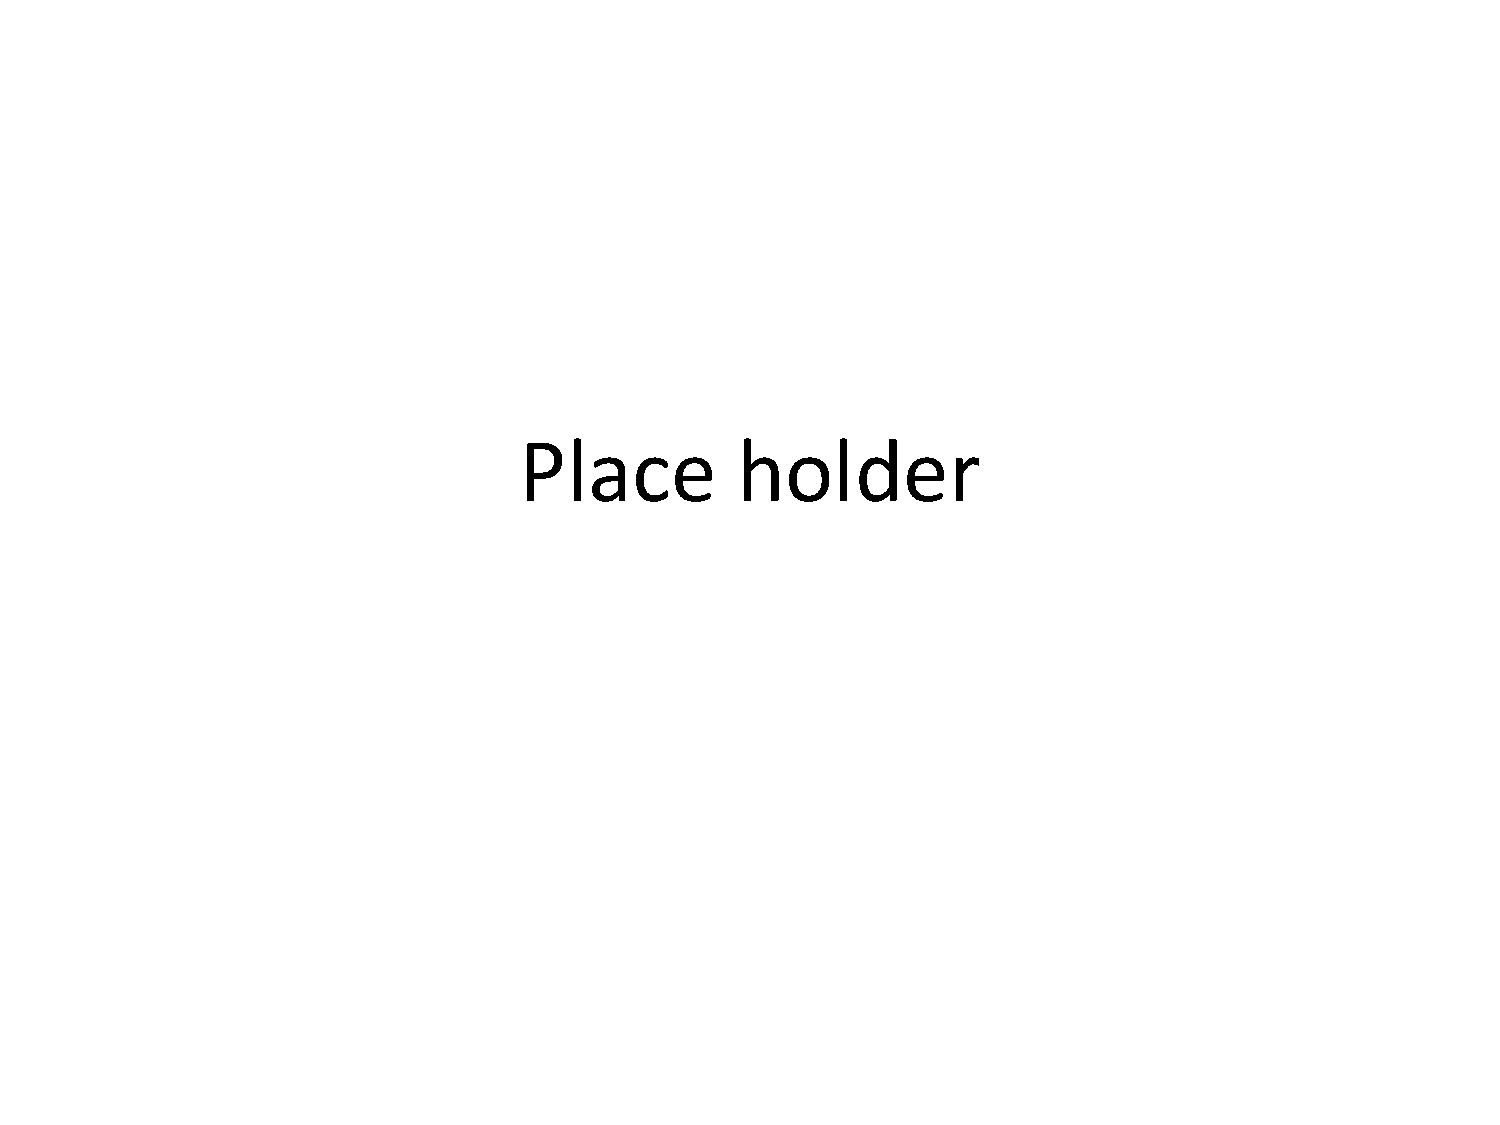
\includegraphics[scale=0.3]{figures/placeHolder}
\caption{Iterates of SQP for Example \ref{ex:cluster nondiff}}
\label{fig:placeholder}
\end{figure}

\end{exmp}

\subsection{Approximating the distance function}
\label{sec:dist smoothing}
The distance function $\dist(\cdot,U)$ is in $L_2(\Re^n)$, so it can be approximated arbitrarily well using a Meyer wavelet expansion~\cite{DeVore_1998}.
%This function is globally Lipschitz with Lipschitz constant 1 and therefore differentiable almost everywhere (Rademacher's theorem), and has a second derivative almost everywhere if $U$ is convex (Alexandrov's theorem) \cite{MakelaN92book}.
%It is well-known that if an a.e.-differentiable function is convolved with a smooth kernel, the output function no longer has those singularities.
%We leverage this to provide a smooth approximation of the distance function by expanding it over a basis of orthonormal Meyer wavelets.
Specifically, the 1-D Meyer wavelet function is given in the frequency domain by ($i = \sqrt{-1})$:
\[\widehat{\psi}(\omega) = \frac{1}{\sqrt{2\pi}} \left \lbrace 
\begin{matrix} \sin (\frac{\pi}{2}\nu(\frac{3|\omega|}{2\pi}-1))e^{i\omega/2} & 2\pi/3 \leq |\omega| \leq 4\pi/3 \\
\cos (\frac{\pi}{2}\nu(\frac{3|\omega|}{4\pi}-1))e^{i\omega/2}, & 4\pi/3 \leq |\omega| \leq 8\pi/3\\
0, &\text{otherwise}\end{matrix} \right. \]
where $\nu(x) = 0$ if $x\leq 0$, $1$ if $x \geq 1$, and equals $x$ if $0\leq x \leq 1$.
The time-domain expression for this wavelet is given in~\cite{Valenzuela15} and is infinitely differentiable.
An $n$-D wavelet can be obtained using the tensor product construction~\cite{DeVore_1998}.
Let $E$ be the set of vertices of the unit hypercube $[0,1]^n$.
For every $e = (e_1,e_2,\ldots,e_n) \in E$ and $x = (x_1,\ldots,x_n) \in \Re^n$, define $\Psi^e:\Re^n \rightarrow \Re$ by $\Psi^e(x)= \psi^{e_1}(x_1)\ldots \psi^{e_n}(x_n)$.
%\begin{equation*}
%\label{eq:tensor meyer}
%\Psi^e(x)= \psi^{e_1}(x_1)\ldots \psi^{e_n}(x_n)
%\end{equation*}
Given $k \in \Ze$ and $\mathbf{j} \in \Ze^n$, a \textit{dyadic cube} in $\Re^n$ is a set of the form $I = 2^{-k}(\mathbf{j} + [0,1]^n)$.
Let $D$ be the set of all dyadic cubes in $\Re^n$ obtained by varying $k$ over $\Ze$ and $\mathbf{j}$ over $\Ze^n$.
Then $\{\Psi^e_{I}, e \in E, I\in D\}$ is an orthonormal basis for $L_2(\Re^n)$ (because the Meyer wavelet itself is orthonormal).
Then every function in $L_2(\Re^n)$ has an expansion 
\[f(x) = \sum_{I \in D} \sum_{e \in E} c_I^e \Psi^e_I(x), \, c_I^e \defeq\, \langle f,\Psi^e_I \rangle\]
with $\langle h,g \rangle \defeq \int_{\Re^n}h(x)g(x)dx$.
The desired approximation is obtained by truncating this expansion after a finite number of terms, i.e., by using  a \textit{finite} set $D' \subsetneq D$
\begin{equation}
\dist(x,U) \approx \sdist_\varepsilon(x,U) \defeq \sum_{I \in D'} \sum_{e \in E} c_I^e \Psi^e_I(x)
\end{equation}
where $\varepsilon$ is the approximation error magnitude.
Using more coefficients yields a better approximation.
The coefficients $c_I^e \defeq\, \langle \dist(\cdot, U), \Psi^e_I \rangle$ are calculated offline and stored in a lookup table for online usage.


%The Meyer scaling function is given in the frequency domain by 
%\[\widehat{\varphi}(\omega) = \frac{1}{\sqrt{2\pi}} \left \lbrace 
%\begin{matrix} 1 & |\omega| \leq 2\pi/3 \\
%                     \cos[\frac{\pi}{2} \nu(3|\omega|/2\pi -1)], & 2\pi/3 \leq |\omega| \leq 4\pi/3\\
%                     0, &\text{otherwise}\end{matrix} \right. \]
%where $\nu(x) = 0$ if $x\leq 0$, $1$ if $x \geq 1$, and equals $x$ if $0\leq x \leq 1$.

%They are used extensively in signal processing, because their approximation properties can be tailored to the class of functions being approximated - e.g., hyperbolic wavelets are suitable for approximating functions of mixed smoothness, such as the distance function we are interested in~\cite{Heping04_HyperbolicWav}.
%In our case, since we know the singularity lines of $\dist$, we can use a directional wavelet basis, and orient it locally such that it has slow variation along the singularity line, and fast variation accross it.


%We give an example of such a construction, which lays the groundwork for explaining the more general wavelet-based smoothing we use in the experiments.
%$C^\infty(\Re^n)$ is the class of functions that are infinitely differentiable in $\Re^n$.
%\begin{theorem}
%	\label{thm:ge smoothing}
%	Consider the globally Lipschitz function $f:\Re^n \rightarrow \Re$ with Lipschitz constant $L_f$.
%	Let $g: \Re^n \rightarrow \Re_+$ be a non-negative $C^\infty(\Re^n)$ function that integrates to 1 and is supported on the unit ball:
%	$\int_{\Re^n}g(x)dx = 1$, $g(x) = 0$ if $x \notin B(0,1)$.
%	Define $g_\varepsilon = \varepsilon^{-n}g(x/\varepsilon)$ and
%	\[f_\varepsilon(x) = f *g_\varepsilon(x) = \int_{\Re^n}f(y)g_\varepsilon(x-y)dy\]
%	Then $\fe$ is infinitely differentiable, its Lipschitz constant $L_{\fe} \leq L_f$ and $\|f-\fe\|_\infty \leq L_f \varepsilon$.
%\end{theorem}
%\begin{proof}
%	Clearly, $\fe$ is $C^\infty$: $g_\varepsilon \in C^\infty$ and the integrand in the above convolution is differentiable w.r.t. $x$, so it holds that $\fe'(x) = \int{f(y)\partial g_\varepsilon(x-y)/\partial x dy}$.
%	
%	Convolution is commutative so $f_\varepsilon(x) = \int_{\Re^n}f(x-y)g_\varepsilon(y)dy$.
%	Let $x' \in \Re^n$, then 
%	\begin{eqnarray*}
%	|\fe(x)-\fe(x')| &=& |\int_{\Re^n} f(x-y)g_\varepsilon(y) - f(x'-y)g_\varepsilon(y) dy|
%	\\
%	&\leq & \int_{\Re^n} g_\varepsilon(y)|f(x-y) - f(x'-y)| dy
%	\\
%	& = & L_f|x-x'| \int_{\Re^n} \varepsilon^{-n} g(y/\varepsilon) dy
%	\\
%	&= &L_f|x-x'| \int_{\Re^n} \varepsilon^{-n} g(y') \varepsilon^ndy'
%	\\
%	&=& L_f|x-x'| \implies L_f \leq L_{\fe}
%	\end{eqnarray*}
%	
%	Finally, 
%	\begin{eqnarray*}
%	|\fe(x)-f(x)| &=& \left|\int_{\Re^n}f(x-y)g_\varepsilon(y)dy - \int_{\Re^n}f(x)g(y)dy\right|
%	\\
%	&=& \left|\int_{\Re^n}f(x-\varepsilon y)g(y)dy - \int_{\Re^n}f(x)g(y)dy\right|
%	\\
%	&\leq& \int_{B(0,1)}|f(x- \varepsilon y) - f(x)|g(y)dy	
%	\\
%	&\leq & \int_{B(0,1)}L_f | \varepsilon y| g(y)dy \leq L_f \varepsilon
%	\end{eqnarray*}
%	In particular, $\|f-\fe\|_\infty \rightarrow 0$ as $\varepsilon \rightarrow 0$.
%\end{proof}
%Fig.~\ref{fig:smooth2d} shows the distance function $\dist(\cdot,U)$ where $U$ is a square in the plane, smoothed by convolving with kernel $g_{\varepsilon}$ obtained from the shown function. 
%We used $\varepsilon = 0.001$, and the actual approximation error $\|f-\fe\|_\infty$ is less than 1e-15.
%Parameter $\varepsilon$ controls how peaked or flat $g_\varepsilon$ is: a large $\varepsilon$ gives a peaked kernel which yields better local approximation, but the max error decreases towards 0 slower.
%
%\begin{figure}[t!]
%	\centering
%	\begin{subfigure}[t]{0.25\textwidth}
%		\includegraphics[height=1.2in]{figures/smoothedSignedDist}
%		\caption{Smoothed function}
%	\end{subfigure}%
%	~
%	\begin{subfigure}[t]{0.25\textwidth}
%		\includegraphics[height=1.2in]{figures/kernelG}
%		\caption{Function $g$}
%	\end{subfigure}
%	\caption{{\small Smoothed 2-d  (negative) signed distance function to a square in the x-y plane, and the function $g$ used to smoothen it.}}
%	\vspace{-10pt}
%	\label{fig:smooth2d}
%\end{figure}


\subsection{Smooth max and min}
\label{max min smoothing}
The following standard smooth approximations of $m$-ary max and min are used.
Let $k \geq 1$.
\begin{eqnarray}
	\label{eq:soft max min}
	\smax_k(a_1,\ldots,a_m) &\defeq& \frac{1}{k} \ln(e^{ka_1}+\ldots+e^{ka_m})
	\\
	\smin_k(a_1,\ldots,a_m) &\defeq& -\smax(-a_1,\ldots,-a_m)
\end{eqnarray}
Suppose $k=1$ and that $a_1$ is the largest number.
Then $e^{a_1}$ is even larger than the other $e^{a_i}$'s, and dominates the sum. 
Thus $\smax_1(\mathbf{a}) \approxeq \ln e^{a_1} = a_1 = \max(\mathbf{a})$.
If $a_1$ is not significantly larger than the rest, the sum is not well-approximated by $e^{a_1}$ alone.
To counter this, the scaling factor $k$ is used: it amplifies the differences between the numbers.
It holds that for any set of $m$ reals,
\begin{eqnarray}
\label{eq:smooth max error}
0 \leq \smax_k(a_1,\ldots,a_m) -\max(a_1,\ldots,a_m) \leq \ln(m)/k
\\
0 \leq \min(a_1,\ldots,a_m) -\smin_k(a_1,\ldots,a_m) \leq \ln(m)/k
\end{eqnarray}
with the maximum error is achieved when all the $a_i$'s are equal.
Indeed, assume $a_1$ is the largest number, then 
$\smax_k(\mathbf{a}) - a_1 \leq k^{-1}\ln\left(\frac{\sum_ie^{ka_i}}{e^{ka_1}}\right) \leq \ln m /k$.

%Indeed, the error of smooth max can be bounded as follows.
%Assume $a_1$ is the largest number, then 
%\begin{eqnarray*}
%\varepsilon_M &\defeq& \smax_k(\mathbf{a}) - a_1 =  \frac{\ln(\sum_ie^{ka_i})-ka_1}{k}
%\\
%&=& k^{-1}\ln\left(\frac{\sum_ie^{ka_i}}{e^{ka_1}}\right) \leq k^{-1}\ln \left(\frac{me^{ka_1}}{e^{ka_1}}\right)
%\\
%&=&\frac{\ln m}{k}
%\end{eqnarray*}
%It is also clear from what preceded that $\varepsilon_M \geq 0$.

\subsection{Overall approximation}
\label{sec:overall apx}
Putting the pieces together, we obtain the approximation error for the robustness of any MTL formula.
\begin{theorem}
	\label{thm:total apx error}
	Consider an MTL formula $\formula$ and reals $\varepsilon > 0$ and $k \geq 1$. 
	Define the \textit{smooth robustness} $\srobf$, obtained by substituting $\mathbf{dist}_\varepsilon$ for $\mathbf{dist}$, $\smax_k$ for $\max$, and $\smin_k$ for $\min$, in Def. \ref{def:robustness estimate}.
	Then for any length-$N$ trajectory $\sstraj$, it holds that
	\[|\robf-\srobf| \leq \delta_\formula\]
	where $\delta_\formula$ is (a) non-negative, 
	(b)independent of the evaluation time $t$, and 
	(c) goes to 0 as $\varepsilon \rightarrow 0$ and $k \rightarrow \infty$.
%	\[|\robf-\srobf| \leq |\formula| \cdot \max(\varepsilon,\ln(m)/k)\]
%	where $m$ is the length of the longest temporal interval appearing in $\formula$ and $|\formula|$ is the size of the formula, i.e. the number of operators that appear in it.
\end{theorem}
\begin{proof}
	We will prove a stronger result that implies the theorem.	
%	Define $\delta_\formula \in \Re_+$ inductively: 
%	$\delta_\top = 0, \delta_p = \varepsilon$, $\delta_{\neg \formula} = \delta_\formula$, 
%	$\delta_{\formula_1 \lor \formula_2} = \delta_{\formula_1 \land \formula_2} = \delta_{\formula_1} \sqcup \delta_{\formula_2} + \ln(2)/k$,
%	$\delta_{\formula_1 \until_{[a,b]} \formula_2}  = \delta_{\formula_1} \sqcup \delta_{\formula_2} + \ln(b-a)/k$.
%	Noting that $\delta_\formula \leq |\formula| \cdot \max(\varepsilon,\ln(m)/k)$, it suffices to show that the error is upper-bounded by $\delta_\formula$.
	When $\sstraj$ or $t$ are clear from the context, we will drop them from the notation.
	
	The proof is by structural induction on $\formula$, and works by carefully characterizing the approximation error.
	The case $\formula = \top$ is trivial.
	
\underline{Case $\formula = p \in AP$.}
$\robf(\sstraj,t)$ is given by either $\dist{x_t}{\Oc(p)}$ or $-\dist{x_t}{\Oc(p)}$, and 
$\srobf(\sstraj,t)$ is given by either $\sdist(x_t,\Oc(p))$ or $-\sdist(x_t,\Oc(p))$, respectively.
Either way, $|\srobf(\sstraj,t) - \robf(\sstraj,t)| \leq \varepsilon$.
Indeed, $\varepsilon$ satisfies the conditions on $\delta_\formula$.

\underline{Case $\formula = \neg \formula_1$} 
$|\rob_{\neg \formula_1}(\sstraj,t)-\srob_{\neg \formula_1}(\sstraj,t)| = |-\rob_{\formula_1}(\sstraj,t) + \rob_{ \formula_1}(\sstraj,t)|  \leq \delta_{\formula_1}$, and $\delta_{\formula_1}$ satisfies (a)-(c) by induction hypothesis.

\underline{Case $\formula = \formula_1 \lor \formula_2$}.
If the same sub-formula $\formula_i$ achieves the max for both $\rob_{\formula_1}(\sstraj,t) \sqcup \rob_{\formula_2}(\sstraj,t)$ and $\srob_{\formula_1}(\sstraj,t) \sqcup \srob_{\formula_2}(\sstraj,t)$, then by induction hypothesis we immediately obtain 
$|\robf(\sstraj,t)-\srob(\sstraj,t)|  \leq \delta_{\formula_i} \leq \delta_{\formula}$.

Otherwise if, say, $\robf = \rob_{\formula_1}$ and $\srobf = \srob_{\formula_2}$ then
\[\robfa -\delta_{\formula_1} \leq \srob_{\formula_1} \leq \srob_{\formula_2} \implies \robfa-\srob_{\formula_2} \leq \delta_{\formula_1}\]
Also 
\[\srob_{\formula_2} \leq \robfb+\delta_{\formula_2} \leq \robfa + \delta_{\formula_2} \implies -\delta_{\formula_2} \leq \robfa - \srob_{\formula_2}\]
Therefore
\begin{equation*}
\label{eq:inter}
-(\delta_{\formula_1} \sqcup \delta_{\formula_2})\leq \robfa - \srob_{\formula_2}\leq \delta_{\formula_1} \sqcup \delta_{\formula_2} \Leftrightarrow |\robfa - \srob_{\formula_2}|\leq \delta_{\formula_1} \sqcup \delta_{\formula_2}
\end{equation*}
Similarly, if $\robf = \rob_{\formula_2}$ and $\srobf = \srob_{\formula_1}$, we have $|\robfb - \srob_{\formula_1}|\leq  \delta_{\formula_1} \sqcup \delta_{\formula_2}$.
So in all cases, 
\[|\robfa \sqcup \robfb - \srob_{\formula_1} \sqcup \srob_{\formula_2}|\leq \delta_{\formula_1} \sqcup \delta_{\formula_2}\]
Therefore 
\[|\robfa \sqcup \robfb - \smax_k(\srob_{\formula_1} , \srob_{\formula_2})|\leq  \delta_{\formula_1} \sqcup \delta_{\formula_2} + \ln(2)/k  = \delta_\formula\]
Clearly, $\delta_\formula$ satisfied (a)-(c).

The case $\formula_1 \land \formula_2$ is treated similarly.

\underline{$\formula = \formula_1 \until_I \formula_2$.} 
Before proving this case, we will need the following lemma, which is provable by induction on $n$:
\begin{lemma}
	\label{lemma:n-ary apx}
	If $\formula = \formula_1\land \ldots\land \formula_n$ or $\formula = \formula_1\lor \ldots\lor \formula_n$, $n\geq 2$, then 
	$|\robf - \srobf| \leq \sqcup_{1\leq i \leq n}\delta_{\formula_i} + \ln(n)/k$.
\end{lemma}

We now proceed with the proof of the last case.
Recall that $\rob_{ \formula_1 \until_I \formula_2} (\sstraj,t) = \sqcup_{t' \in t+_{\TDom}I} \left(\rob_{\formula_2} (\sstraj,t') \bigsqcap \right.
\\
\left. \sqcap_{t'' \in [t,t')}   \rob_{\formula_1} (\sstraj,t'') \right)$.
Starting with the innermost sub-expression $\rob_\psi \defeq \sqcap_{t'' \in [t,t')}   \rob_{\formula_1} (\sstraj,t'')$, we have, by Lemma \ref{lemma:n-ary apx}
\begin{equation}
\label{eq:robpsi}
|\rob_{\psi}-\srob_\psi| \leq \sqcup_{t'' \in [t,t')}\delta_{\formula_1}^{t''} + \ln(t'-t)/k
\end{equation} 
where $\delta_{\formula_1}^{t''} $ is the bound for approximating $\rob_{\formula_1}(\sstraj,t'')$.
But $\delta_\formula$ does not depend on the time at which the formula is evaluated. Therefore the bound in \eqref{eq:robpsi} becomes
\begin{equation*}
|\rob_{\psi}-\srob_\psi| \leq \delta_{\formula_1} + \ln(t'-t)/k
\end{equation*} 
%
To avoid introducing a dependence on time, we further upper-bound by 
\begin{equation*}
|\rob_{\psi}-\srob_\psi| \leq \delta_{\formula_1} + \ln(hrz(\formula))/k \defeq \delta_\psi
\end{equation*} 
where, recall, $hrz(\formula)$ is the horizon of $\formula$ (see Section \ref{sec:mtl}).

Continuing with the sub-expression $\rob_\alpha = \rob_{\formula_2} (\sstraj,t') \bigsqcap \rob_\psi$, by the induction hypothesis it holds that 
$|\rob_\alpha - \srob_\alpha| \leq \delta_{\formula_2} \sqcup \delta_\psi + \ln(2)/k \defeq \delta_\alpha$.
%
Finally, the top-most max operator introduces the total error 
\begin{eqnarray*}
|\robf-\srobf| &\leq& \delta_\alpha + \ln(|I|)/k 
\\
&=& \delta_{\formula_2} \sqcup \delta_\psi + \ln(2)/k + \ln(|I|)/k 
\\
&=& \delta_{\formula_2} \sqcup ( \delta_{\formula_1} + \ln(hrz(\formula))/k )+ \ln(2|I|)/k 
\\
&=&\delta_\formula
\end{eqnarray*}
The first inequality obtains from the fact that $\delta_\alpha$ is independent of evaluation time and Lemma \ref{lemma:n-ary apx}.
The bound $\delta_\formula$ obey s (a)-(c).
This concludes the proof.
%if $\formula_1$ is a sub-formula of $\formula$, then $\delta_{\formula_1} \leq \delta_\formula$.
	\end{proof}

\section{Approximation error and control}
\label{sec:examples}
We implemented the smooth approximation to the semantics of MTL, and tested it empirically on several examples.

\subsection{Approximation error for robustness}
\label{sec: ex apx error}
\begin{figure}[t]
\centering
\includegraphics[width=0.49\textwidth]{figures/RobustnessError}
\vspace{-30pt}
\caption{{\small RMSE (and variance) of robustness approximation error against formula horizon, evaluated on 1000 randomly generated trajectories for the system in \eqref{eq:PointMass}. Unless noted, the states in the trajectory are in $\mathbb{R}^2$. Note, the magnitude of the approximation errors are very small, as is the variance, showing the accuracy of the smooth approximation of robustness.}}
\vspace{-10pt}
\label{fig:sample result}
\end{figure}

We evaluated the robustness $\robf$ and its approximation $\srobf$ for five formulae, with $hrz(\formula_i) = N$. $P_1$ and $P_2$ are atomic propositions for state being in two different polyhedra.
%Each formula is of the form $\formula_i = \always_{[0:N-1]} \psi$, where $N$ is the length of the trajectory.
%Thus $hrz(\formula_i)  = N$.
Each formula's robustness is evaluated on 1000 randomly-generated trajectories of varying lengths $N$, so we can  examine the error's variation with the horizon.
The trajectories were produced by a 2-or-3 dimensional system, \eqref{eq:PointMass} with input and state saturation.
%All formulas use the atomic propositions $P_1 \defeq x \in [-1,1]^n$ and $P_2 \defeq x\in [2,2.5]^n$, where $n = 2,3$ is the dimension of the system.
%The state-space is $[-5,5]^n$ and the input set is $\inpSet = [-0.3,0.3]^n$. 

Fig. \ref{fig:sample result} shows the Root Mean Square (RMSE) of the approximation, $\sqrt{(1/1000)\sum_{\sstraj}(\robf(\sstraj)-\srobf(\sstraj))^2}$
, and variance bars around it. 
As seen, the approximation error is small for all cases.
Note that while the RMSE  increased with the system dimension ($4^{th}$ formula in Fig.~\ref{fig:sample result}), it was observed that the relative error remained very small i.e. the increase in error is explained by an increase in the robustness's magnitude. 

%As suggested by Remark \ref{rem:upper bound}, the approximation error generally increases with the horizon (for a constant number of wavelet coefficients).
%This is due to the smooth max and min functions, as seen in \eqref{eq:smooth max error}.
%Fig. \ref{fig:relative error} shows the relative approximation errors, $(\robf-\srobf)/|\robf|$, for the formulae under consideration. 
%It is seen that the average relative approximation error is less than $10\%$ for all cases. 
%For some data points in Fig. \ref{fig:relative error}, the variance of relative error is high, but the error remains small in absolute terms as seen in Fig.~\ref{fig:sample result}.

%In general, the high relative approximation errors are due to trajectories which have a true robustness of near zero; 
%these lead to a spike in the relative approximation error, $(\robf-\srobf)/|\robf|$, even for small values of the absolute error $|\robf-\srobf|$.


%\begin{figure}[t]
%\centering
%\includegraphics[width=0.49\textwidth]{figures/RobustnessErrorRel}
%\vspace{-30pt}
%\caption{{\small Mean and variance of relative approximation error against formula horizon, evaluated on 1000 randomly generated trajectories for the system in \eqref{eq:PointMass}. Unless noted, the states in the trajectory are in $\mathbb{R}^2$.}} 
%\todo[inline]{smae changes as previous fig. All temporal operators must be bounded}}
%\label{fig:relative error}
%\vspace{-15pt}
%\end{figure}

%\vspace{-30pt}
\subsection{Robustness maximization for control}
\label{sec:toy example}
To solve Problem $P_\rob$ given in \eqref{eq:general_ctrl}, we replace the true robustness $\robf$ by its smooth approximation $\srobf$.
We thus obtain Problem $P_{\srob}$.
We illustrate the approach on a simple linear system,
and provide more extensive case studies in Section \ref{sec:case study}.

\subsubsection{Illustrative example}
\label{sec:illustrative example}
We consider a linear system with the following dynamics:
\begin{equation}
\label{eq:PointMass}
x_{k+1} = x_k + u_k
\end{equation}

The specification is 
\[\formula = \always_{[0,20]} \neg (x_k \in \text{Unsafe}) \land \eventually_{[0,20]} (x_k \in \text{Terminal})\]
with the sets $\text{Unsafe}=[-1,1]^2$ i.e. a hyper-cube in $\mathbb{R}^2$ with length 2, centered on the origin) and $\text{Terminal}=[2,2.5]^2$. 
The state space is $X=[-2.5,2.5]^2$, $U=[0.3,0.3]^2$, $\delta=1$, and we optimize for two different values of $\gamma$, $0.1$ and $0.001$. 
The initial point of the optimization is $x_0=[-2,-2]'$. 
The control cost is $l(x_k,u_k) = ||x_k||_{2}^2$, so that $\sum_kl(x_k,u_k)$ penalizes the length of the trajectory. Here, $hrz(\formula) = 21$.

\textbf{Optimization solver.}
We use Sequential Quadratic Programming (SQP) to solve the optimization problem $P_{\srob}$.
SQP solves constrained non-linear optimization problems, like $P_{\srob}$, by creating a sequence of quadratic approximations to the problem and solving these approximate problems.
SQP enjoys various convergence-to-(local)-optima properties, depending on the assumptions we place on the problem. 
See \cite[Section 2.9]{Polak97_Optim}.
For example, for SQP to converge to a strict local minimum (a minimum that is strictly smaller than any objective function value in an open neighborhood around it), it suffices that 
1) all constraint functions be twice Lipschitz continuously differentiable. 
In our case, this includes function $f$ in \eqref{eq:general ctrl obj}, and the problems we solve satisfy this requirement.
%We will need to assume that $f$ is twice Lipschitz continuously differentiable and that its gradient $f_u$ has maximum row rank.
And, 
2) at points in the search space that lie on the boundary of the inequality-feasible set (where the inequality constraints are satisfied with equality), there exists a search direction towards the interior of the feasible set that does not violate the equality constraints (the so-called Mangasarian-Fromowitz constraint qualification) \cite[Assumption 2.9.1]{Polak97_Optim}.
This is also true in our case since our equality constraints come from the dynamics and are always enforced for any $\mathbf{u}$.

\textbf{Solver initialization}.
To initialize SQP (i.e., give it a starting point for the optimization), we need an \textit{initial trajectory} that starts from $x_0$. We can obtain this initial trajectory:

 a) The standard way, by solving a feasibility linear program with constraints \eqref{eq:general ctrl dyn}-\eqref{eq:general ctrl U}. By definition, the solution to a feasibility program is a trajectory that simply satisfies the constraints without optimizing the objective. This is in general a computationally lightweight solution as the optimization being solved is a simple linear program.
 
 b) By randomly generating an input sequence (which respects the bounds on the input/states). Such a trajectory will be fast to generate and feasible w.r.t the dynamics but is unlikely to satisfy the specification on the system. 

Note, the initial trajectory is free to violate the specification (as it does in every example we study in this paper) and we only enforce that it needs to satisfy the dynamics and constraints of the system which we are controlling.

%In most cases, SQP solvers can also recover from infeasible starts, that is the initial trajectory can also violate the dynamics and constraints of the system, but at the cost of computation effort, hence we enforce the feasibility constraint on the initial trajectory.

\textbf{Results}.
Fig.~\ref{fig:toy control} shows the sets, initial trajectory (which is unsafe and has a robustness of $-1$), and two trajectories obtained by solving $P_{\srob}$ for two different values of $\gamma$ (with $\delta=0$). Both trajectories satisfy the specification $\formula$. Intuitively, the trajectories in Fig.\ref{fig:toy control} make sense, as for a higher value of $\gamma=0.1$ we get a shorter trajectory, which is closer to unsafe set, hence satisfies $\formula$ less robustly ($\rob_{\formula}=0.65$) and for a smaller value of $\gamma=0.001$ we get a longer trajectory with a higher robustness ($\rob_{\formula}=1.21$).

\textbf{Comparison to BluSTL.}
We also compare the timing and robustness maximization performance for our method with BluSTL \cite{}. BluSTL has two modes of operation, \textit{boolean}: which aims at satisfying the specification (we set control cost to zero), and \textit{robust}: which uses a MILP encoding of robustness and attempts to maximize it (again we set control cost to zero). For a fair comparison of our method to BluSTL, we emulate the \textit{boolean} mode of BluSTL by terminating the optimization at the iteration of SQP where $\srob \geq \epsilon_{\text{Meyer}}$. The \textit{robust} operation is obtained by solving $P_{\srob}$ until SQP terminates (on a local minima, possibly global). Similar to the optimization cost of BluSTL, we set $\gamma=0$ in $P_{\srob}$ for both modes, i.e. no control cost. All methods are run in a \textit{one-shot} manner, that is a single optimization is solved at time step $0$ to get a trajectory with a length of $N$ time steps, where $hrz(\formula) = N$.

We run 100 instances with the specification and dynamics of our illustrative example, with a random initial state $x_0 \in [-2.5,-1.5] \times [-2.5,2.5]$ for each instance. We also vary the formula horizon (and hence optimization length of the trajectory being optimized over) $N$ from $20$ to $200$ time-steps. Table \ref{tbl:time_performance_toy} shows the execution times for each method and the two modes of operation. All experiments were run on a machine with a quad-core Intel I5 3.2GHz processor with 24GB RAM, running MATLAB 2016b.


\begin{table}[tb]
\small
\begin{center}
\caption{{\small Runtimes (mean and standard, in seconds) for Smooth Operator (SR-SQP) and BluSTL (BlS) over 100 runs with random initial states and with different formula horizon lengths $N$. Here, (B) means \textit{boolean} mode and (R) means \textit{robust} mode of operation.}}
\vspace{-5pt}
\label{tbl:time_performance_toy}
\begin{tabular} {|c|c|c|c|c|}
	\hline
	N & BlS(B) & SR-SQP(B) & BlS(R) & SR-SQP(R) \\ \hline
	20 & $0.96 \pm 0.82$ &  $\mathbf{0.31 \pm 0.13}$  & NA & $3.30 \pm 1.25$ \\ \hline
	30 & $1.37 \pm 1.72$ &  $\mathbf{0.33 \pm 0.25}$  & NA & $5.85 \pm 2.74$\\ \hline
	40 & $3.86 \pm 5.10$ &  $\mathbf{0.60 \pm 0.29}$  & NA & $12.36 \pm 6.04$\\ \hline
	50 & $4.36 \pm 12.97$&  $\mathbf{0.74 \pm 0.30}$ & NA & $30.05 \pm 18.23$\\ \hline
	100& $16.77 \pm 27.84$ & $\mathbf{1.21 \pm 0.25}$ & NA & $69.70 \pm 13.16$ \\ \hline
	200& $53.88 \pm 14.18$& $\mathbf{4.19 \pm 1.18}$ & NA & $126.11 \pm 20.43$ \\ \hline
\end{tabular}	
\end{center}
\end{table}

\textbf{Analysis.}
As seen in table \ref{tbl:time_performance_toy}, our method is consistently faster than BluSTL for the \textit{boolean} mode, and also displays smaller variances in runtimes. For BluSTL in \textit{robust} mode, BluSTL could not finish a single instance of robustness maximization within 100 hours on both the machine used for running experiments as well as on a machine with 8 core Intel Xeon machine with 60GB RAM, leading us to believe that the problem formulation in BluSTL did not scale into a tractable MILP. Note, the problem solved here is very similar to the example used in \cite{Saha_acc16}, which uses another MILP based method to find satisfying trajectories. While the underlying dynamics and the machine on which evaluations are run are different, these results suggest that our run-times compare favourably with those in \cite{Saha_acc16}.

When in \textit{boolean} mode, BluSTL results in trajectories with zero robustness (as seen in), while our method results in trajectories with an average robustness of 0.10. Both methods satisfy $\formula$ in all 100 instances. In \textit{robust} mode, across all experiments, SR-SQP results in an average $\rob_{\formula}=0.247$ with a standard deviation of less than $0.005$. It is to be noted, that an upper bound on the maximum achievable $\rob_{\formula}$ is $0.25$, which can be achieved by trajectory reaching (in number of time steps $\leq N$) the point $[2.25,2.25]$ in the middle of the Terminal set while always avoiding the Unsafe set by a distance greater than $0.25$. This shows that for this problem, our method reaches very close to achieving the global optima of $\rob_{\formula}$. Also with this additional knowledge of the global optima upper bound, the SR-SQP method in \textit{robust} mode can be made a lot faster by specifying an exit condition based on a upper threshold of $\srob_{\formula}$ attained at any iteration of the SR-SQP method. While for brevity we do not include results with this additional stopping criteria, it was observed that for an upper bound value of $\srob_{\formula}=0.24$, an average speed up of about $4$-times was observed for $N=20$ and $2$-times for $N=200$ while resulting an average robustness value achieved of $\rob_{\formula} = 0.235$. This shows that with the iterative nature of SQP, we can trade-off performance for improved execution times.

\textbf{Note} that in BluSTL, atomic propositions in general have to be of the form $a'x\leq b$ (although absolute value and polynomials are also valid) since robustness is encoded as a MILP, which necessitates avoiding the signed distance function in dimensions greater than 1. This implies that atomic propositions in higher dimensions ($x\in \mathbb{R}^{n>1}$), $Hx \leq g$, have to be broken down into the conjunction of $n$ individual atomic propositions of the form $h_i'x \leq g_i$. This also restricts atomic propositions in BluSTL from involving sets like circles or ellipsoids. On the other hand, atomic propositions in our work can involve non-Polyhedron sets (e.g. ellipsoids or circles) and even non-convex sets since we do not avoid the signed distance function for higher dimensions.

\begin{figure}[t]
\centering
\includegraphics[width=0.49\textwidth]{figures/ToyExampleControl}
\vspace{-30pt}
\caption{{\small Initial trajectory and trajectories obtained for two different values of $\gamma$ in \eqref{eq:general_ctrl}.}}
\label{fig:toy control}
\vspace{-10pt}
\end{figure}


%%Toy Falsification example
\todo[inline]{skipping for now}
We can also formulate a falsification problem \cite{AbbasATVA11_LinFalsification}, \cite{AbbasF_HybridSA12}, \cite{Deshmukh15_IterativeApproaches} by minimizing robustness in order to find trajectories of a closed loop system that violate a specification. In particular, we solve the following problem:

\begin{subequations}
\label{eq:falsification}
\begin{align}
\text{min}&_{x_0 \in X_0 } \, \rob_{\Psi}(\sstraj) \nonumber \\
\text{s.t. } & x_{k+1} = f_k(x_0) \, \forall k=0,\dotsc,N-1 \\
&  x_{k} \in X \, \forall k=1,\dotsc,N
\end{align}
\end{subequations}

For evaluation, we solve the problem for the point-mass system of \eqref{eq:PointMass}, with a state feedback controller for fixed-point tracking to the state $[2.25\,2.25]'$, which lies in the middle of the Terminal set (Fig. \ref{fig:toy falisification}). The specification is $\Psi=\always_{[0,20]} \neg (x_k \in \text{Unsafe})$, where the set $\text{Unsafe}$ is as defined earlier. The set of possible initial state, $X_0$ is shown in Fig. \ref{fig:toy falisification}, as is the initial point (used for initialization in the optimizer) and resulting trajectory, which satisfies $\Psi$ with a robustness of $1.25$. As before, $N=20$ is the length of the resulting trajectory under consideration.

For evaluation, we compare A) SQP using smooth robustness, B) SQP using Robustness and C) Simulated Annealing \cite{SABOOK}. Initial states and trajectories from the 3 methods are shown in Fig.\ref{fig:toy falisification}. Here. methods A) and B) result in the same initial state $x_0=[-2.3418\, -2.3418]'$, while C) gives $x_0=[-2.3371\, -2.3354]'$. The robustness for trajectories from both SQP based methods is $-0.99998$, while via Simulated Annealing is $-0.9968$. Note, the trajectories via either method are very close, and pass near the center of the $\text{Unsafe}$ set (the origin), where the robustness reaches its minima of $-1$. Also worth noting, that for the trajectory via method A), $\srob_{\Psi}=-0.9932$, i.e. a relative approximation error of less than $1\%$.

\begin{figure}[t]
\centering
\includegraphics[width=0.49\textwidth]{figures/ToyExampleFalse}
\caption{Trajectories from initial points obtained from robustness minimization via Simulated Annealing (SA), SQP, and SQP on smooth robustness. Note, both SQP and SQP on smooth robustness lead to the same solution.}
\label{fig:toy falisification}
\end{figure}
\section{Case study}
\label{sec:case study}
\todo[inline]{introduce two numerical examples. Finite horizon control in a single shot, can be applied in a receding/shrinking horizon approach wherever applicable.}


\subsection{HVAC Control of a building for comfort}
%caseBldg

In order to evaluate the control performance of our method on a system with more meaningful dynamics than the point-mass system, we test it on temperature control of a 4-state model of a single zone room in a building (\cite{HAMLAB}). Such a model is commonly used in literature for evaluation of predictive control algorithms \cite{AchinACC}. The control problem we solve is similar to the example used in \cite{Raman14_MPCSTL}, where the objective is to bring the room temperature to a comfortable range when the building is occupied (given predictions on the building occupancy). The specification is gives as:
\begin{equation}
\label{eq:BldgSpec}
\Psi = \always_I(\text{RoomTemp} \in \text{Comfort})
\end{equation}
Here, $I$ is the interval where the room is occupied, and $\text{Comfort}$ is the range of temperatures (in Celsius) deemed comfortable ($[22,28]$). For the control horizon, we consider a 24 hour period, in which the building is occupied from time steps $10$ to $19$ (i.e. $I=[10,19]$), corresponding to a 10-hour workday. The single-zone model, discretized at a sampling rate of 1 hour (which is common in building temperature control) is of the form:

\begin{equation}
x_{k+1} = Ax_{k}+Bu_k+B_dd_k
\end{equation}
Here, $A$, $B$ and $B_d$ matrices are from the HAMLAB model. $x \in \mathbb{R}^4$ is the state of the model, the $4^{th}$ element of which is the room temperature, the others are auxiliary temperatures corresponding to other physical properties of the zone. The input to the system, $u \in \mathbb{R}^1$ is the heating/cooling energy to the system. $b_d \in \mathbb{R}^3$ are disturbances (due to occupancy, outside temperature, solar radiation), which we assume perfect predictions of. Data for the disturbances is obtained for $1^{st}$ April 2000, which is our 24 hours of interest, from the ??? data set. The control problem we solve is of the form in \eqref{eq:general_ctrl}, with $\gamma$ and $\delta$ both set to zero, i.e. robustness is only in the objective, to be maximized. This allows for a fair comparison between our method (SQP on smooth robustness), gradient descent (SQP) on robustness, and Simulated Annealing (SA) for robustness maximization. With respect to the general control problem of \eqref{eq:general_ctrl}, the limits on the states are $X=[0,50]^4$ and on the inputs $U=[-1000,2000]$.

To initialize the optimzation for all three methods, we generate an initial trajectory, starting from $x_0=[21 \, 21 \, 21 \, 21]'$, which does not satisfy $\formula$. The trajectories after optimization from the three methods are shown in Fig.\ref{fig:ZoneTemp}. Our method and SA both result in trajectories that satisfy $\formula$, with a robustness of $2.9994$ and $2.8862$ respectively. On the other hand, SQP for gradient descent on the robustness function results in a trajectory that does not satisfy $\formula$ ($\rob_{\formula} = -0.1492$), and terminates on a local maxima. This is possibly due to the lack of existence of a gradient along certain directions. 

In the particular problem, with the given comfort range, the maximum robustness achievable in the unconstrained case would $3$, achieved by setting the room temperature at $25$C for the interval $I$. Our method results in a robustness which is just $0.02\%$ less than the unconstrained optimal value, while SA gets to a value $3.8\%$ less than the (unconstrained) optima. Note, for this particular problem, since we assume perfect knowledge of occupancy and disturbances, the problem of satisfying the formula, or indeed of even maximizing robustness, can be solved simply with a quadratic program with linear constraints. We use this example to illustrate the applicability of our method, as well as its performance, while adding a word of caution against the naive use of gradient descent for robustness maximization, even while the gradient of robustness exists \textit{almost everywhere}. In the following example, we take a specification which cannot be trivially turned into a quadratic-program without adding tighter constraints than the specification asks for (or binary variables).


\begin{figure}[t]
\centering
\includegraphics[width=0.49\textwidth]{figures/ZoneTemp_scissored}
\caption{Zone temperatures. The green rectangle shows the comfortable temperature limit of 22-28 C, applicable during time steps 10-19 (when the building is occupied).}
\label{fig:ZoneTemp}
\end{figure}

%1. Single zone building model from ...

%2. Specification for comfort when occupied.

%3. 24 hour look ahead, given disturbances and occupancy. Initial guess (with negative robustness) via solving an LP.

%4. Can be applied in a receding horizon manner. For the given setting, could very well be solved using a linear program asking for temperature between 22-28C for time steps 10 to 19, but we use our method to illustrate how robustness based control can be used to satisfy a specification. The next example (Autonomous ATC) shows control with a specification cannot be trivially translated to a linear program with Polyhedral constraints.

%5. Figure shows room temperature for the 3 methods (other states and disturbances/control in a single figure if necessary)

%6. Table shows robustness of obtained trajectory via the 3 methods. Note, Optimal solution would be temperature of 25C  (robustness of 3) for the occupancy period (if dynamics/constraints would allow it).



\subsection{Autonomous Air Traffic Controller for quad-rotors}
%CaseQuad
\todo[inline]{Start by motivating the example as something more than a dumb system. E.g. "Air traffic control offers many opportunities for automation to allow a more efficient and safer landing patterns. The constraints of air traffic control are complex and contain many safety rules. In this example we express these rules in MTL and demonstrate how the smoothed robustness is used to generate control strategies for safely and robustly landing two quadrotors. The proposed approach outperforms Simulated Annealing and gradient descent on the non-smooth robustness."
	
	Then you give the details below}
1. We take a quad-rotor model with linearized dynamics around hover, similar to those used in \cite{}. The case study involves centralized control of two quad-rotors, with operational objectives given as an MTL specification, and a constrained air-space.

1.b. Give model, constraints, specification. Shrinking horizon (fixing history) approach applicable (cite Vasu paper)

2. With the given specification, standard control approaches involving polyhedral constraints are hard to apply because of the temporal aspect of the eventually operator involved. While the two (if-then) altitude rules in the specification can be coded as polyhedral constraints on the set, it would result in a non-convex constraint set for positions. Similarly, the minimum distance between two quad-rotors can also be moved to the constraints but would result in another non-convex constraint if we choose to do so. In our formulation, the non-convexity remains in the cost-function while the constraints are linear.

3. For simulation purposes, we use obtain 3 initial trajectories (via solving different linear programs) from the given initial state to the terminal (landing) set. These three trajectories, each of which has negative robustness (i.e. does not satisfy the given specification), serve as three different initial solutions to A) Our approach B) SQP using the actual robustness function as the cost, C) Simulated Annealing with the actual robustness function as the cost. This multi-start approach can be used in practice when there is a fast initial trajectory generator available.

3.b. parameters for simulation annealing and citation for it.

4. Fig shows the initial trajectories for both the quadrotors in the given air-space. Fig. shows the three trajectories obtained after applying our control method, with the three initial trajectories as starting points for the optimization, respectively. 

5. Table shows for the three trajectories, initial robustness, robustness for trajectory obtained via the three methods (and the approximate robustness when applicable). In addition, we also tested out simulated annealing with the smooth robustness function in the cost (with the first initial trajectory), resulting in a trajectory with a final cost of blah (approximate robustness of blah).



\begin{figure}[t]
\centering
\includegraphics[width=0.49\textwidth]{figures/QuadInitTrajs_scissored}
\caption{The airspace with the corresponding sets, and initial trajectories for the two quad-rotors. Note, all 3 initial trajectories violate the specification. Here, $p0_{i}^j$ refers to the positions of the $i^{th}$ initial trajectory for the $j^{th}$ quadrotor.}
\label{fig:quad_init}
\end{figure}

\begin{figure}[t]
\centering
\includegraphics[width=0.49\textwidth]{figures/QuadTrajs_scissored}
\caption{ Trajectories obtained via SQP on smooth robustness, with three different initial trajectories acting as initial solutions for the SQP. Note, all 3 trajectories satisfy $\Psi$. Here, $p_{i}^j$ refers to the positions of the $i^{th}$ initial trajectory for the $j^{th}$ quadrotor.}
\label{fig:quad_init}
\end{figure}


\subsection{Discussion}
With a simple 2-state numerical example, and two case studies on systems with more complex dynamics, we show the applicability and consistently good performance of our method. As seen in the two case studies, our method outperforms both simulated annealing and gradient descent (via SQP) on the robustness function. Also, while in the first case study, gradient descent does not find a trajectory that satisfies the specification, in the second case study, simulated annealing cannot find trajectories that satisfy the specification from two of the three initial trajectories (used as initial solutions for optimization). Our method on the other hand, successfully finds a trajectory that satisfies the specification, while resulting in the best robustness value achieved across all examples considered. 
Since all implementations were done in MATLAB, the focus was not real-time applicability of the proposed method. For the first case study, where the dynamics are slow, our method should still be applicable ($~20s$) of execution time (compared to $~5 \text{ mins}$ for SA), for the second case study a MATLAB implementation is infeasible due to the very fast dynamics and sampling times involved. We have shown previously in ??? that control of a real quadrotor with the dynamics in \eqref{eq:quad_dyn} is possible on a low computation power platform while solving multiple quadratic programs at even higher sampling rates ($20Hz$). With this in mind, we expect a C/C++ implementation of SQP (and the smooth robustness function) should allow us to implement our method on such a system. Ongoing work focuses on a general interpreter for formulae to generate corresponding smooth robustness functions, as well as their derivatives.
%\addtolength{\textheight}{-12cm}   % This command serves to balance the column lengths
% on the last page of the document manually. It shortens
% the textheight of the last page by a suitable amount.
% This command does not take effect until the next page
% so it should come on the page before the last. Make
% sure that you do not shorten the textheight too much.
\bibliographystyle{plain}
\bibliography{iccps2017,hscc17,hscc2016,fainekos_bibrefs}
\end{document}